% ==================================================
% Anhang
% --------------------------------------------------

\newappendix{Interviewleitfaden für das Interview mit Christian Krauthoff}
\label{Interviewleitfaden für das Interview mit Christian Krauthoff}

\todo[color=TODO]{Intervierwleitfaden schreiben}
\begin{tabular}{|p{10cm}|p{4cm}|}
    \hline
    \textbf{Interviewfragen} & \textbf{Bezugskapitel} \\
    \hline
    1. Frage 1 & Kapitel 1 \\
    \hline
    2. Frage 2 & eigene Ergänzung \\
    \hline
    \end{tabular}

\newpage

\newappendix{Interviewprotokoll 1: Christian Krauthoff}\label{appendix: Anhang 3}

\todo[color=REVIEW]{Daten überprüfen}
\begin{tabular}{p{2.5 cm}p{11.8 cm}}
\textbf{Protokoll:} & Gespräch mit Christian Krauthoff \\
\textbf{Teilnehmer:} & Christian Krauthoff - Abteilungsleiter AZV \& ZV-Rekla (OE-4293) \break Tobias Binnewies - Dualer Student \\
\textbf{Thema:} & Produktionsdatenspeicherung / Transaktionskosten / Großrechner \\
\textbf{Dauer:} & 30 min
\end{tabular}
\bigbreak
\noindent\rule[1ex]{\textwidth}{1pt} %Linie
\bigbreak

\textbf{Frage:} 
\phantomsection
\label{i1:f1}
Wie wird sichergestellt, dass Produktionsdaten (bspw. Kontodaten) nicht manipuliert werden können?


\textbf{Antwort:} 
Als Mitarbeiter braucht man ein Produktionsrecht und ein recht sensitive Daten einsehen zu dürfen, um auf die Daten mit einem Auftragsgrund zugreifen zu können. Der Auftragsgrund besteht dann durch ein Ticket, also quasi eine „Beschwerde” durch ein Institut.
Nur dann kann ein FI-Mitarbeiter auf Produktionsdaten zugreifen.
Um Daten abzuändern muss noch ein weiteres Recht beantragt werden, das nur wenige Mitarbeiter haben.
Außerdem kommt das Vieraugenprinzip zum Einsatz, sodass immer mindestens zwei Mitarbeiter mit diesem Recht das SQL-Statement einsehen müssen, bevor es ausgeführt wird.

Source Code wird maschinell geprüft, also bspw. dass keine festen IBANs, Namen oder ähnliches im Code fest abgefragt werden.
Außerdem wird immer ein Code Review von „Unabhängigen„ - also Entwicklern, die an diesem Projekt nicht beteiligt waren - durchgeführt, um so die Qualität des Codes zu gewährleisten.

\bigbreak
\bigbreak

\textbf{Frage:}
\phantomsection
\label{i1:f2}
Wie werden Daten bei Änderung nachvollziehbar gespeichert?


\textbf{Antwort:}
Wenn Daten „gelöscht” werden oder auch geändert werden, werden diese nie wirklich gelöscht sondern nur deaktiviert.
So gibt es bei jeder gespeicherten Zeile in der Datenbank ein Feld „Gültig bis”, welches erst einmal leer ist. 
Ändert sich nun etwas an der Zeile, wird das Feld „Gültig bis” mit dem Datum der Änderung gefüllt und eine neue Zeile mit den neuen Daten wird angelegt.
So ist eine Löschung oder Änderung jederzeit nachvollziehbar.

In der DSGVO ist festgelegt, sind Datenlöschungfristen festgelegt.
Kontodaten haben eine Löschfrist von 10 Jahren, d. h. diese müssen 10 Jahre lang gespeichert werden und können dann erst wirklich gelöscht werden.

\bigbreak
\bigbreak

\textbf{Frage:}
\phantomsection
\label{i1:f3}
Wie hoch sind die Kosten pro Transaktion?


\textbf{Antwort:} 
Die Informationen dazu stehen im Produktkatalog. Außerdem gibt es SQLs, die einem die genauen Kosten für das jeweilige Insitut auswerfen.

Die Kosten für die Finanz Informatik sind pro Transaktion schwer anzugeben, da es sich hierbei um Volumentverträge handelt. 
Hierbei wird eine Lastspitze der Großrechners im gesamten Jahr festgelegt und demnach abgerechnet. 


\bigbreak
\bigbreak

\textbf{Frage:}
\phantomsection
\label{i1:f4}
Gibt es Projekte um vom Großrechner wegzukommen?


\textbf{Antwort:}
Ja, man möchte klar vom Großrechner wegkommen - und auch vorallem von IBM abhängig zu sein.
Es gibt das Projekt „COBOL to Java”, also von COBOL / IBM weg und so nur noch die kritischen Themen dort zu halten, also im Rahmen von Zeit und Massendatenverarbeitung und den Rest alles auslagern in Java.
Allerdings laufen die Java-Jobs zum Teil auch auf dem Großrechner, das Zeil ist jedoch - sofern möglich - die Großrechnerjobs immer weiter zu reduzieren.

Das Problem ist immer die Geschwindigkeit und Massendaten, da dies durch kein anderes System so gut abbildbar ist wie durch den Großrechner.
Bspw. schafft der Großrechner, wenn ein Job mit ca. 1,4 Millionen Transaktionen anstartet ca. 20 Sekunden.
Oder auch wenn z. B. die DKB am Monatsende mit ihren ca. 1,8 Millionen Konten Zinsrechnung, Abschußschreibung oder auch Umbuchung durchführt, laufen mehrere Jobs parallel.
Das ist mit anderen Systemen schwer abbildbar, bzw. auch schnwer einmal zu testen.

\bigbreak
\bigbreak

\textbf{Frage:}
\phantomsection
\label{i1:f5}
Was sind Geschäftsprozesse?


\textbf{Antwort:}
Geschäftsprozesse sind quasi ein „Fahrplan”, dort steht drin, was bspw. von der Erfassung bis zur Buchung mit den Daten passiert, also ob z. B. ob aus 5€ noch 15€ werden, da es noch Gebühren gibt oder ist das nicht erlaubt.
Es wird genau geregelt, welcher Prozess wann, wie und in welcher Reihenfolge abläuft.
So kann genau nachgewiesen werden, was genau mit den Daten passiert ist.
Es gibt dann „Datenflussdiagramme„ für einen genauen Prozess um bspw. bei Beschwerde genau nachvollziehen zu könnne, warum was genau passiert ist.
Es ist technisch nicht möglich einen Prozess zu umgehen, da die Daten immer durch die Prozesse laufen.
Außerdem können bpsw. keine Daten gelöscht oder abgeändert werden, wenn dies nicht im Geschäftsprozess vorgesehen ist.

\newpage

\newappendix{OSPlus-Diagramm}
\phantomsection
\label{a1}
\todo[color=TODO]{Quelle einfügen}
\begin{figure}[ht]
    \centering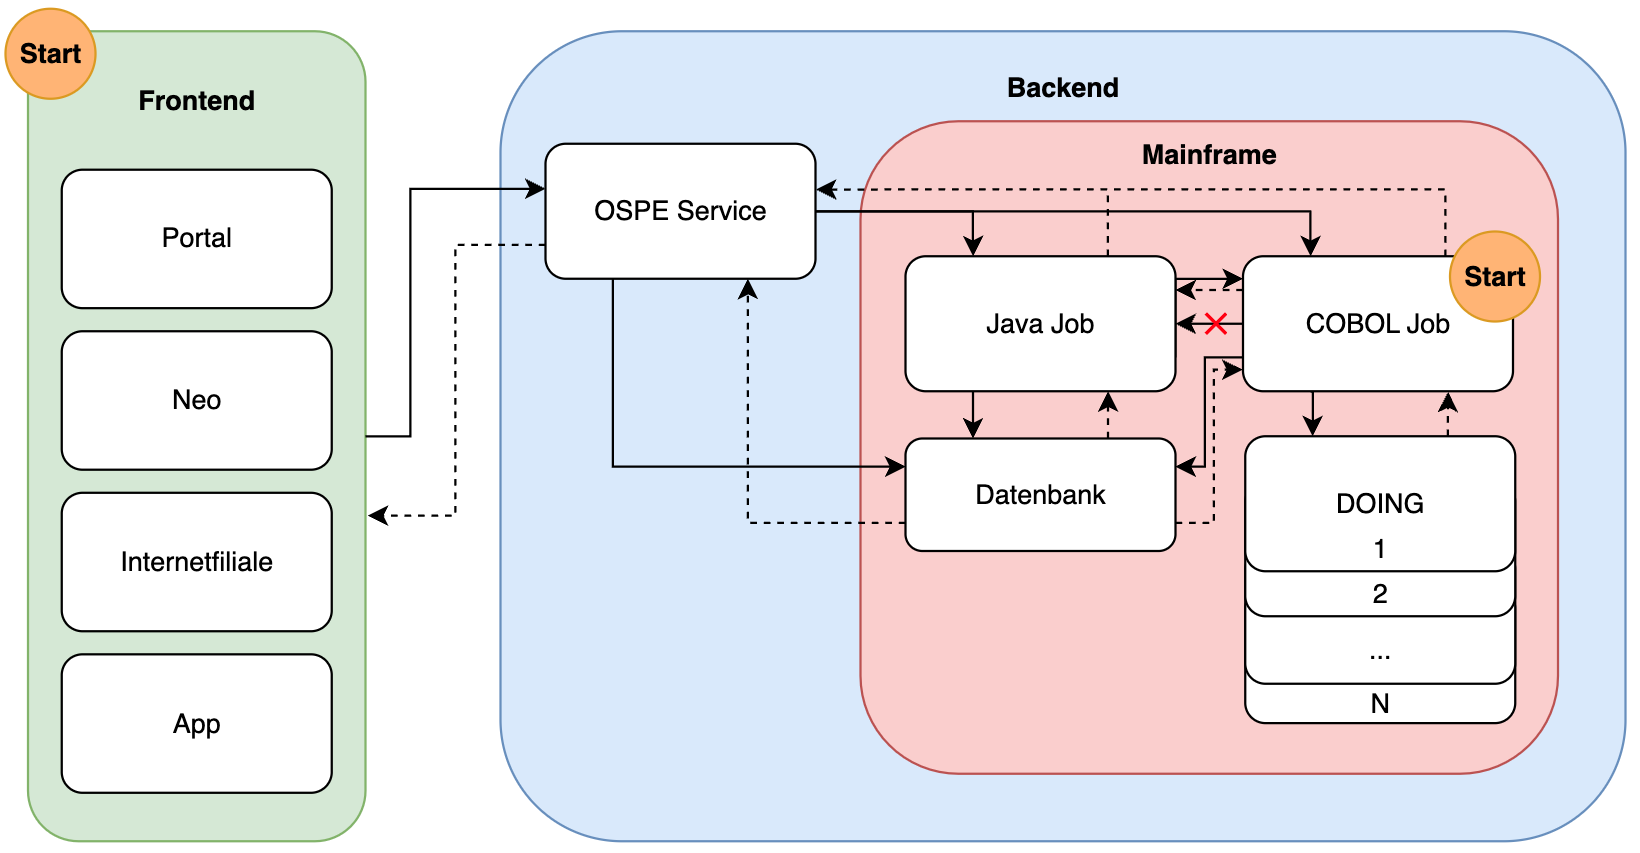
\includegraphics[width=1.0\textwidth]{Abbildungen/OSPlus-Diagramm.png}
\end{figure}

\newpage

\bigbreak